\section{Auswertung}
\label{sec:Auswertung}
\subsection{Messung der Zeitkonstanten $RC$ über die Entladekurve}
Die Entladekurve des $RC$-Kreises wird mit einem Oszilloskop sichtbar gemacht, wie 
in \autoref{fig:aufgabe a - rechteckspannung} zu sehen ist. Die verwendete Frequenz beträgt $f=5\,\symup{kHz}$.
Im Folgenden werden Wertepaare \{$t [\symup{\mu s}], U [\symup{V}]$\} mithilfe von eingezeichneten Hilfslinien abgelesen
(\autoref{fig:aufgabe a - gitter und hilfslinien}) und tabellarisch aufgeführt (\autoref{tab:aufgabe a}). Es ist zu beachten,
dass die Schrittweite von $t$ nicht gleichmäßig gewählt wird, da sich die Werte mit der gewählten Schrittweite mit
geringerem Fehler ablesen lassen. Die Fehler von $t$ und $U$ werden zu
 $\Delta t = 1\,\symup{\mu s}$ und $\Delta U = 0,1\,\symup{V}$ abgeschätzt.

 Die Formel des Entladevorgangs eines Kondensators \autoref{eqn:Entladen} wird umgestellt zu
 \begin{equation}
   \symup{ln}(\frac{U}{U_{0}}) = -\frac{1}{RC}\cdot t.
 \end{equation}
 Mithilfe der Python-Erweiterungen "numpy" \cite{numpy}, \dq scipy" \cite{scipy} und "matplotlib" \cite{matplotlib} werden die Wertepaare der 
 \autoref{tab:aufgabe a} halblogarithmisch geplottet und es wird eine Regressionsgerade ermittelt und eingezeichnet. 

\begin{figure}
  \centering
  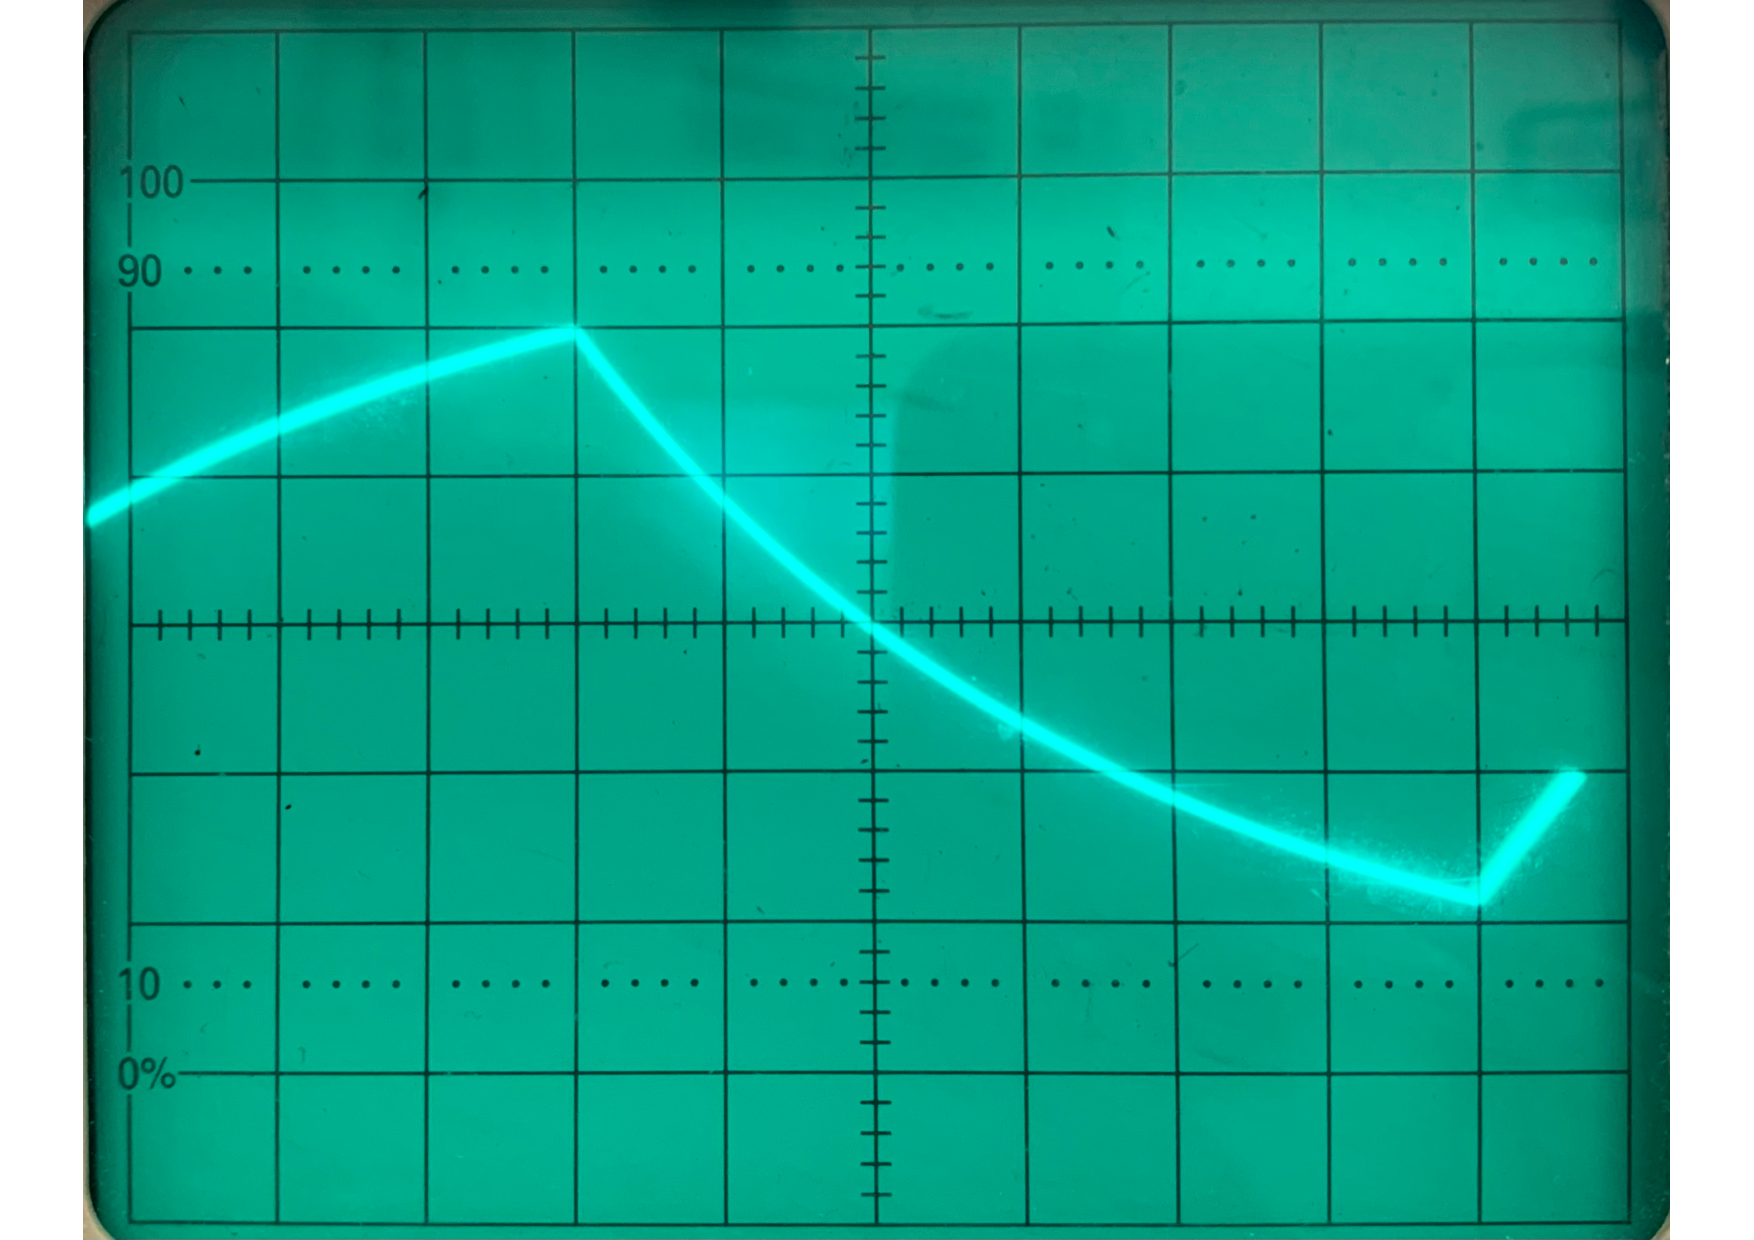
\includegraphics[height=10cm]{content/Aufgabe a - Rechteckspannung.pdf}
  \caption{Entladekurve des Kondensators mit Vorwiderstand.}
  \label{fig:aufgabe a - rechteckspannung}
\end{figure}

\begin{figure}
  \begin{subfigure}{0.48\textwidth}
    \centering
    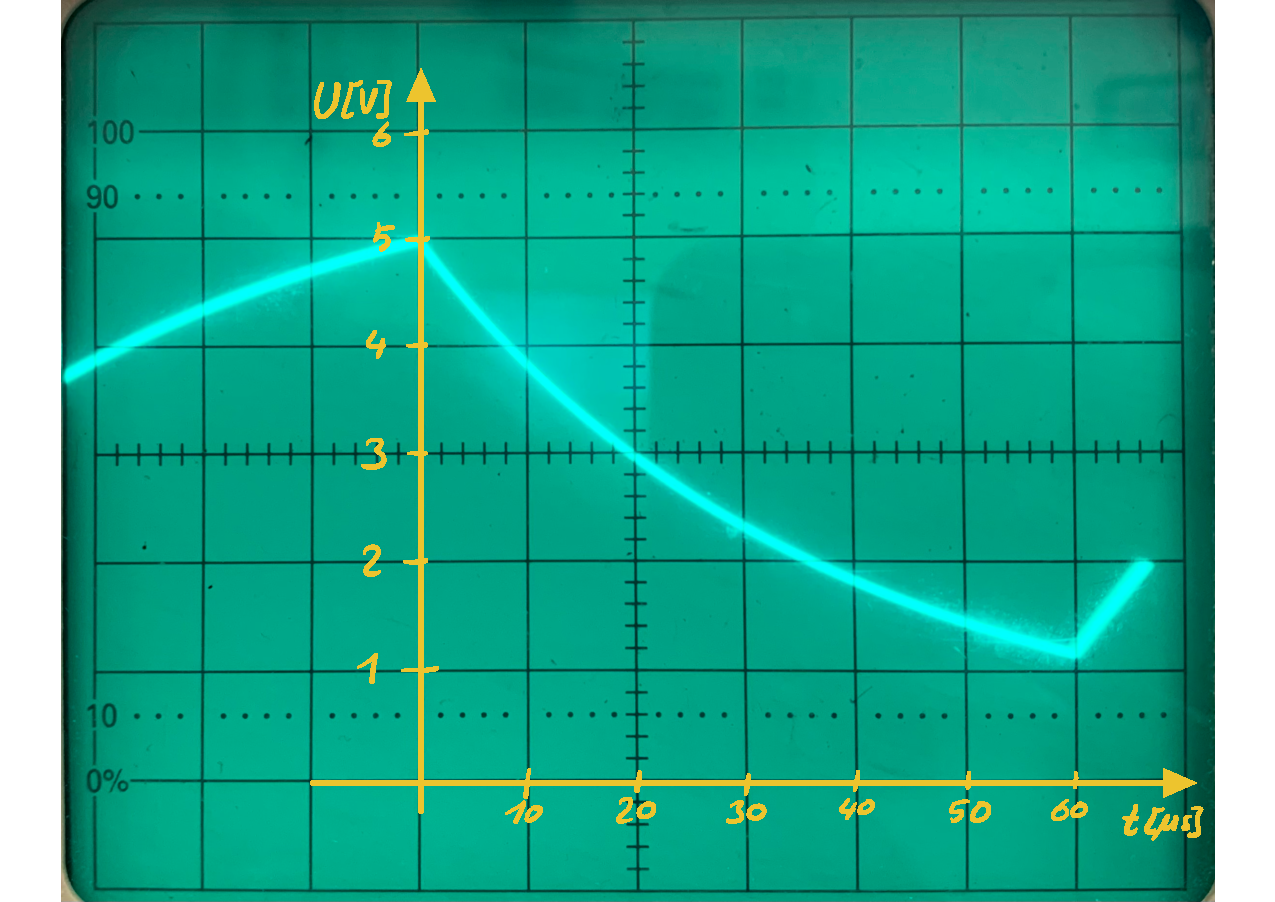
\includegraphics[height=5cm]{content/Aufgabe a - Gitter.pdf}
    \caption{Entladekurve mit Koordinatensystem.}
    \label{fig:aufgabe a - gitter}
  \end{subfigure}
  \hfill
  \begin{subfigure}{0.48\textwidth}
    \centering
    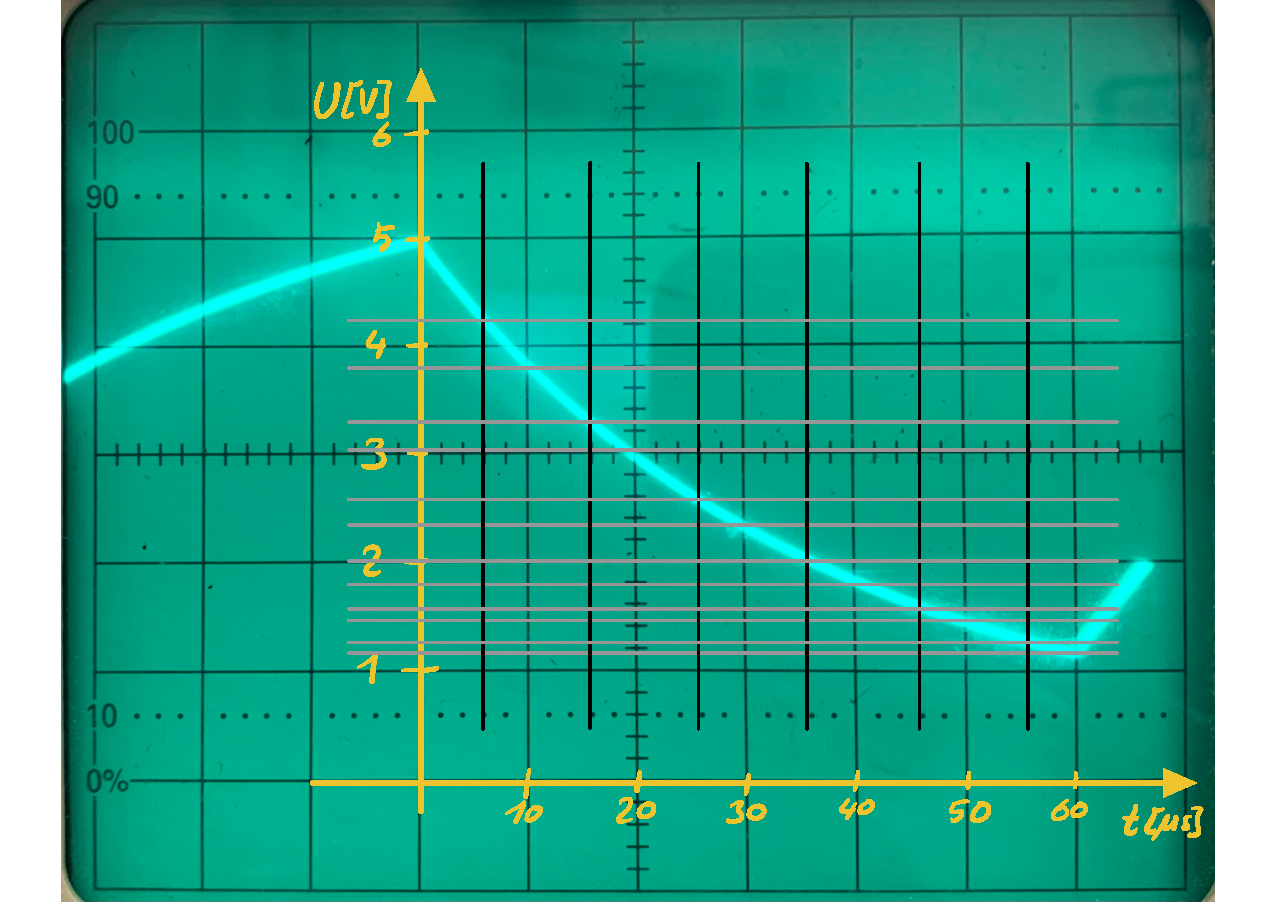
\includegraphics[height=5cm]{content/Aufgabe a - Hilfslinien.pdf}
    \caption{Entladekurve mit Hilfslinien.}
    \label{fig:aufgabe a - hilfslinien}
  \end{subfigure}
  \caption{Entladekurve mit eingezeichnetem Koordinatensystem und Hilfslinien. Die %
    Skalierung wurde vorher durch Abgleich mit der Amplitude der Rechteckspannung ermittelt.}
  \label{fig:aufgabe a - gitter und hilfslinien}
\end{figure}

\begin{table}
  \centering
  \caption{Darstellung der Messwertpaare, welche aus \autoref{fig:aufgabe a - gitter und hilfslinien} abgelesen wurden.}
  \label{tab:aufgabe a}
  \begin{tabular}{S[table-format=2.0] S[table-format=1.1]}
    \toprule
    {$s$ [$\symup{\mu s}$]} & {$U$ [V]} \\
    \midrule
    0 &  5,0 \\
    6	&  4,2 \\
    10 & 3,8 \\
    16 & 3,3 \\
    20 & 3,0 \\
    26 & 2,6 \\
    30 & 2,3 \\
    36 & 2,0 \\
    40 & 1,8 \\
    46 & 1,6 \\
    50 & 1,4 \\
    56 & 1,2 \\
    60 & 1,1 \\
    \bottomrule
  \end{tabular}
\end{table}

\begin{figure}
  \centering
  \includegraphics{build/plot_a.pdf}
  \caption{Halblogarithmischer Plot der Wertepaare aus \autoref{tab:aufgabe a} %
  mit Ausgleichsgerade.}
  \label{fig:plot_a}
\end{figure}



Die Parameter der
Ausgleichsgerade vom Typ $\symup{ln}(\frac{U}{U_{0}}) = m \cdot t + b$ werden zu 
\begin{align}
  m&=-0,02505\pm0,00018\,\unit{\per\second} \\
  b&=0,0136\pm0,0001 \notag
\end{align} 
bestimmt. Unter Benutzung der Gauschen-Fehlerformel...!!!!!!!!!!!!!!!
Die Zeitkonstante $RC$ ist folglich
\begin{gather}
  RC = \frac{1}{m} = (39,92\pm0,28)\,\symup{\mu s}.
\end{gather}



\subsection{Bestimmung der Zeitkonstante $RC$ über die Frequenabhängigkeit der Amplitude}
Die Spannung am Kondensator $A$ wird ebenso wie die Spannung der Sinusspannungsquelle $U_{0}$ bei variabler
Frequenz $f$ gemessen und tabellarisch in \autoref{tab:aufgabe c} dargestellt. Da sich bei der Messung $U_{0}$
als frequenzunabhängig und zu $U_{0} = 2,8$V\footnote{Anm.: Abgelesen wurden 5,2V, allerdings%
ist die Feineinstellung des Oszilloskops defekt, daher konnte die Amplitude nicht kalibriert werden. Für kleine $f$ gilt $U_{0}\approx A$, %
weshalb wir im Folgenden mit $U_{0}=2,8$V gerechnet haben.} bestimmen lässt, ist dieser Wert aus Gründen der
Übersichtlichkeit nicht in der Tabelle aufgeführt. Das Teilungsverhältnis aus $\frac{A}{U_{0}}$ wird berechnet und
gleichermaßen dokumentiert. Als Fehler für die Frequenz $f$ wird $\Delta f = 0,1$Hz und für den Fehler in der Messung
der Amplitude $A$ wird $\Delta A = 0,1$V verwendet.

\begin{table}
  \centering
  \caption{Messwertpaare Frequenz $f$ und Amplitude $A$ sowie die Relativamplitude~$\frac{A}{U_{0}}$.}
  \label{tab:aufgabe c}
  \begin{tabular}{S[table-format=6.0] S[table-format=1.2] S[table-format=1.3]}
    \toprule
    {$f$ [Hz]} & {$A$ [V]} & {$\frac{A}{U_{0}}$} \\
    \midrule
    50     & 2,80	& 1.000 \\
    100    & 2,65 & 0.946 \\
    150    & 2,60  & 0.929 \\
    200    & 2,60  & 0.929 \\
    500    & 2,60  & 0.929 \\
    1000   & 2,50  & 0.893 \\
    1500   & 2,30  & 0.821 \\
    2000   & 2,05 & 0.732 \\
    3000   & 1,80  & 0.643 \\
    4000   & 1,50  & 0.536 \\
    5000   & 1,10  & 0.393 \\
    10000  & 0,68 & 0.243 \\
    20000  & 0,30  & 0.107 \\
    30000  & 0,22 & 0.079 \\
    50000  & 0,14 & 0.050 \\
    100000 & 0,07 & 0.025 \\
    \bottomrule
  \end{tabular}
\end{table}

Die Wertepaare \{$f \symup{[Hz]}, \frac{A}{U_{0}}$\} aus \autoref{tab:aufgabe c} werden in ein Diagramm aufgetragen
und es wird eine nicht-lineare Ausgleichsrechnung mit denselben Python-Erweiterungen wie für die lineare Ausgleichsrechnung
durchgeführt. Auch die Fehlerrechnung wird analog durchgeführt. Für den Plot werden nicht die
gerundeten Werte aus \autoref{tab:aufgabe c} verwendet, sondern die exakteren Werte $\frac{A}{U_{0}}$.

\begin{figure}
  \centering
  \includegraphics{build/plot_b.pdf}
  \caption{Plot der Wertepaare aus \autoref{tab:aufgabe c} mit nicht-linearer Ausgleichsfunktion \autoref{eq:ausgleichsfunktion aufgabe c}.}
  \label{fig:plot_b}
\end{figure}

\begin{figure}[H]
Die nicht-lineare Ausgleichsrechnung liefert für die Funktion 
  \begin{equation}
    \frac{A}{U_{0}} = \frac{1}{\sqrt{1+{\omega}^{2}\cdot (RC)^2}}
    \label{eq:ausgleichsfunktion aufgabe c}
  \end{equation}
den Wert $RC = (68,750206\pm0,000009)\,\symup{\mu s}$.
\end{figure}


% RC_a = 39.92+/-0.28 [\mu s]
% Steigung m: -0.02505+/-0.00018
% Achsenabschnitt b: 1.59580+/-0.00018
% RC_b = [[-68.75020636093754+/-9.24706974716629e-06]] [\mu s]
% RC_c = [[69.01295902314953+/-1.9899821596188524e-05]] [\mu s]

\subsection{Bestimmung der Zeitkonstanten $RC$ über die Frequenzabhängigkeit der Phasenverschiebung%
 zwischen $U_{\symup{C}}$ und $U_{0}$}
 \begin{figure}[H]
  Neben der Amplitude ist auch die Phase zwischen $U_{\symup{C}}$ und $U_{0}$ abhänging von der Frequenz der Spannungsquelle.
  Der Zusammenhang wird durch die Formel
  \begin{equation}
    \varphi(\omega) = -\arctan(-\omega \cdot RC)
    \label{eq:Formel für Phasenverschiebung}
  \end{equation}
  beschrieben. 
 Die Phase $\varphi$ wird über
 \begin{equation}
   \varphi = \frac{a}{b}\cdot 2\symup{\pi}
 \end{equation}
 berechnet. Die Messunsicherheit wird sowohl für $a$ als auch für $b$ mit $\Delta a = \Delta b = 0,1$s berücksichtigt.
 \end{figure}
 
\begin{table} [H]
  \centering
  \caption{Messwert Frequenz $f$, Phasenverschiebung $a$, Periodenlänge $b$. Errechnete Phasenverschiebung $\varphi$.}
  \label{tab:aufgabe d}
  \begin{tabular}{S[table-format=6.0] S[table-format=3.1] S[table-format=5.0] S[table-format=1.3] S[table-format=1.3]}
    \toprule
    {$f$ [Hz]} & {$a$ [$\symup{\mu}$s]} & {$b$ [$\symup{\mu}$s]} & {$\varphi$ [rad]}%
     & {$\varphi$ [$\frac{\symup{\pi}}{\symup{rad}}$]}\\
    \midrule
    50      & 0	  & 20000 & 0.000 & 0.000 \\
    100     & 100 & 10000 & 0.063 & 0.020 \\
    150     &	100 & 6500  & 0.097 & 0.031 \\
    200     &	100 & 5000  & 0.126 & 0.040 \\ 
    500     &	100	& 2000  & 0.314 & 0.100 \\
    1000    &	100 & 1000  & 0.628 & 0.200 \\
    1500    & 55  & 630   & 0.549 & 0.175 \\
    2000    &	50  & 500   & 0.628 & 0.200 \\
    3000    & 44  & 330   & 0.838 & 0.267 \\
    4000    & 40  & 250   & 1.005 & 0.320 \\
    5000    & 36  & 200   & 1.131 & 0.360 \\
    10000   & 22  & 100   & 1.382 & 0.440 \\
    20000   & 12  & 52    & 1.450 & 0.462 \\
    30000   & 8   & 34    & 1.478 & 0.471 \\
    50000   & 4,9 & 20    & 1.539 & 0.490 \\
    100000  &	2,5 & 10    & 1.571 & 0.500 \\
    \bottomrule
  \end{tabular}
\end{table}

\begin{figure} [H]
  \centering
  \includegraphics{build/plot_c.pdf}
  \caption{Plot der Wertepaare aus \autoref{tab:aufgabe d} mit nicht-linearer%
   Ausgleichsfunktion \autoref{eq:Formel für Phasenverschiebung}.}
  \label{fig:plot_c}
\end{figure}

Auch hier wird für die Wertepaare \{$f \symup{[Hz]}, \varphi$ [rad]\} eine nicht-lineare Ausgleichsrechnung unter 
der Funktion für die Phasenverschiebung (\autoref{eq:Formel für Phasenverschiebung}) durchgeführt. Die Zeitkonstante $RC$ lässt 
sich hier bestimmen zu:
\begin{gather}
  RC = (69,01295\pm0,00001)\,\symup{\mu s}.
\end{gather}

Darüber hinaus werden die Messwerte der frequenzabhängigen Amplitude $A$ aus \autoref{tab:aufgabe c} und der
ebenfalls frequenzabhängigen Phase $\varphi$ aus \autoref{tab:aufgabe d} in einem Polarplot (\autoref{fig:plot_d})
visualisiert.
Zum Vergleich wird deren theoretischer Zusammenhang ebenfalls geplottet, dieser ergibt sich aus \autoref{eq:Formel für Phasenverschiebung}
umgestellt nach $\omega$:
\begin{equation}
  \omega = -\frac{\tan(\varphi)}{RC}
\end{equation}
eingesetzt in
\begin{equation}
  A(\omega) = -\frac{\sin(\varphi)}{\omega RC}
\end{equation}
Daraus resultiert
\begin{equation}
  A(\varphi) = \cos (\varphi) \cdot U_{0}.
\end{equation}.


\begin{figure} [H]
  \centering
  \includegraphics{build/plot_d.pdf}
  \caption{Polarplot der Amplitude $A$ in Abhängigkeit der Phasenverschiebung~$\varphi$.}
  \label{fig:plot_d}
\end{figure}

\subsection{Nutzung des $RC$-Kreises zur Integration von Spannungen hoher Frequenz}
Aus \autoref{sec:theorie-integration} wird klar, dass ein $RC$-Kreis Spannungen für eine Frequenz $f >> \frac{1}{RC}$
integriert. Als Erstes wird eine Rechteckspannung angelegt. Der Spannungsverlauf einer Rechteckspannung ist jeweils für ein
Zeitintevall konstant, somit ist eine Stammfunktion dazu von linearer Art, wie auch in \autoref{fig:aufgabe d - rechteckspannung}
zu sehen ist.

Für eine angelegte Dreieckspannung wird erwartet, dass sich für die Spannung $U_{\symup{C}}$ ein quadratischer Verlauf ergibt,
da eine Dreieckspannung für ein Zeitintevall linear steigt oder sinkt. Dies lässt sich auch in \autoref{fig:aufgabe d - dreieckspannung}
erkennen.

Als letztes wird eine Sinusspannungsquelle verwendet. Die Spannung $U_{\symup{C}}$ stellt sich als phasenverschoben
und amplitudenreduziert gegenüber der Spannung $U_{0}$ ein (\autoref{fig:aufgabe d - sinusspannung}). Da eine
Stammfunktion zu der Funktion $f(\omega)=\symup{sin}(\omega t)$ die Funktion $F(\omega) = \frac{1}{\omega}\symup{cos}(\omega t)$ ist,
zeigt sich auch hier, dass der $RC$-Kreis für bestimmte Frequenzen als Integrator dienen kann.

\begin{figure}
  \centering
  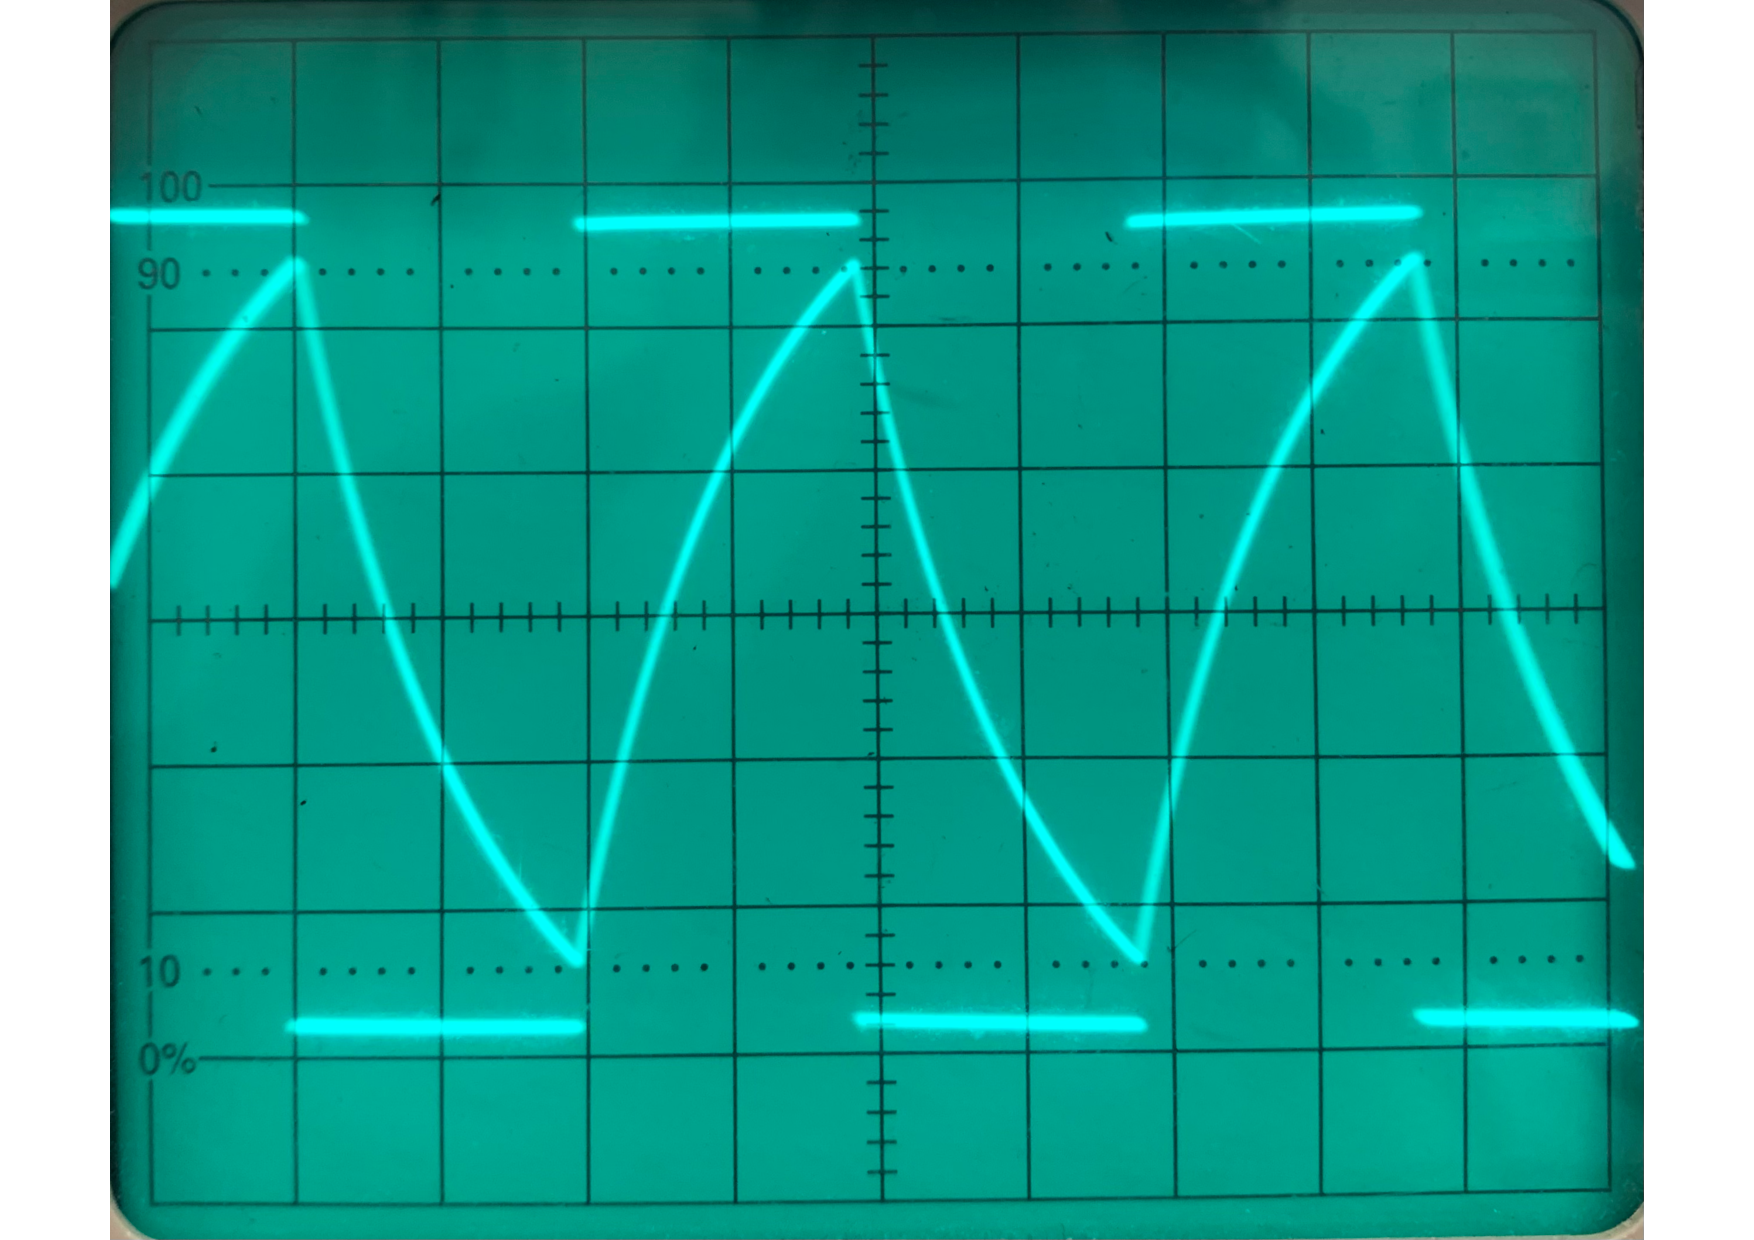
\includegraphics[height=8cm]{content/Aufgabe d - Rechteckspannung.pdf}
  \caption{Rechteckspannung $U_{0}$ und Kondensatorspannung mit $f=5$kHz.}
  \label{fig:aufgabe d - rechteckspannung}
\end{figure}

\begin{figure}
  \centering
  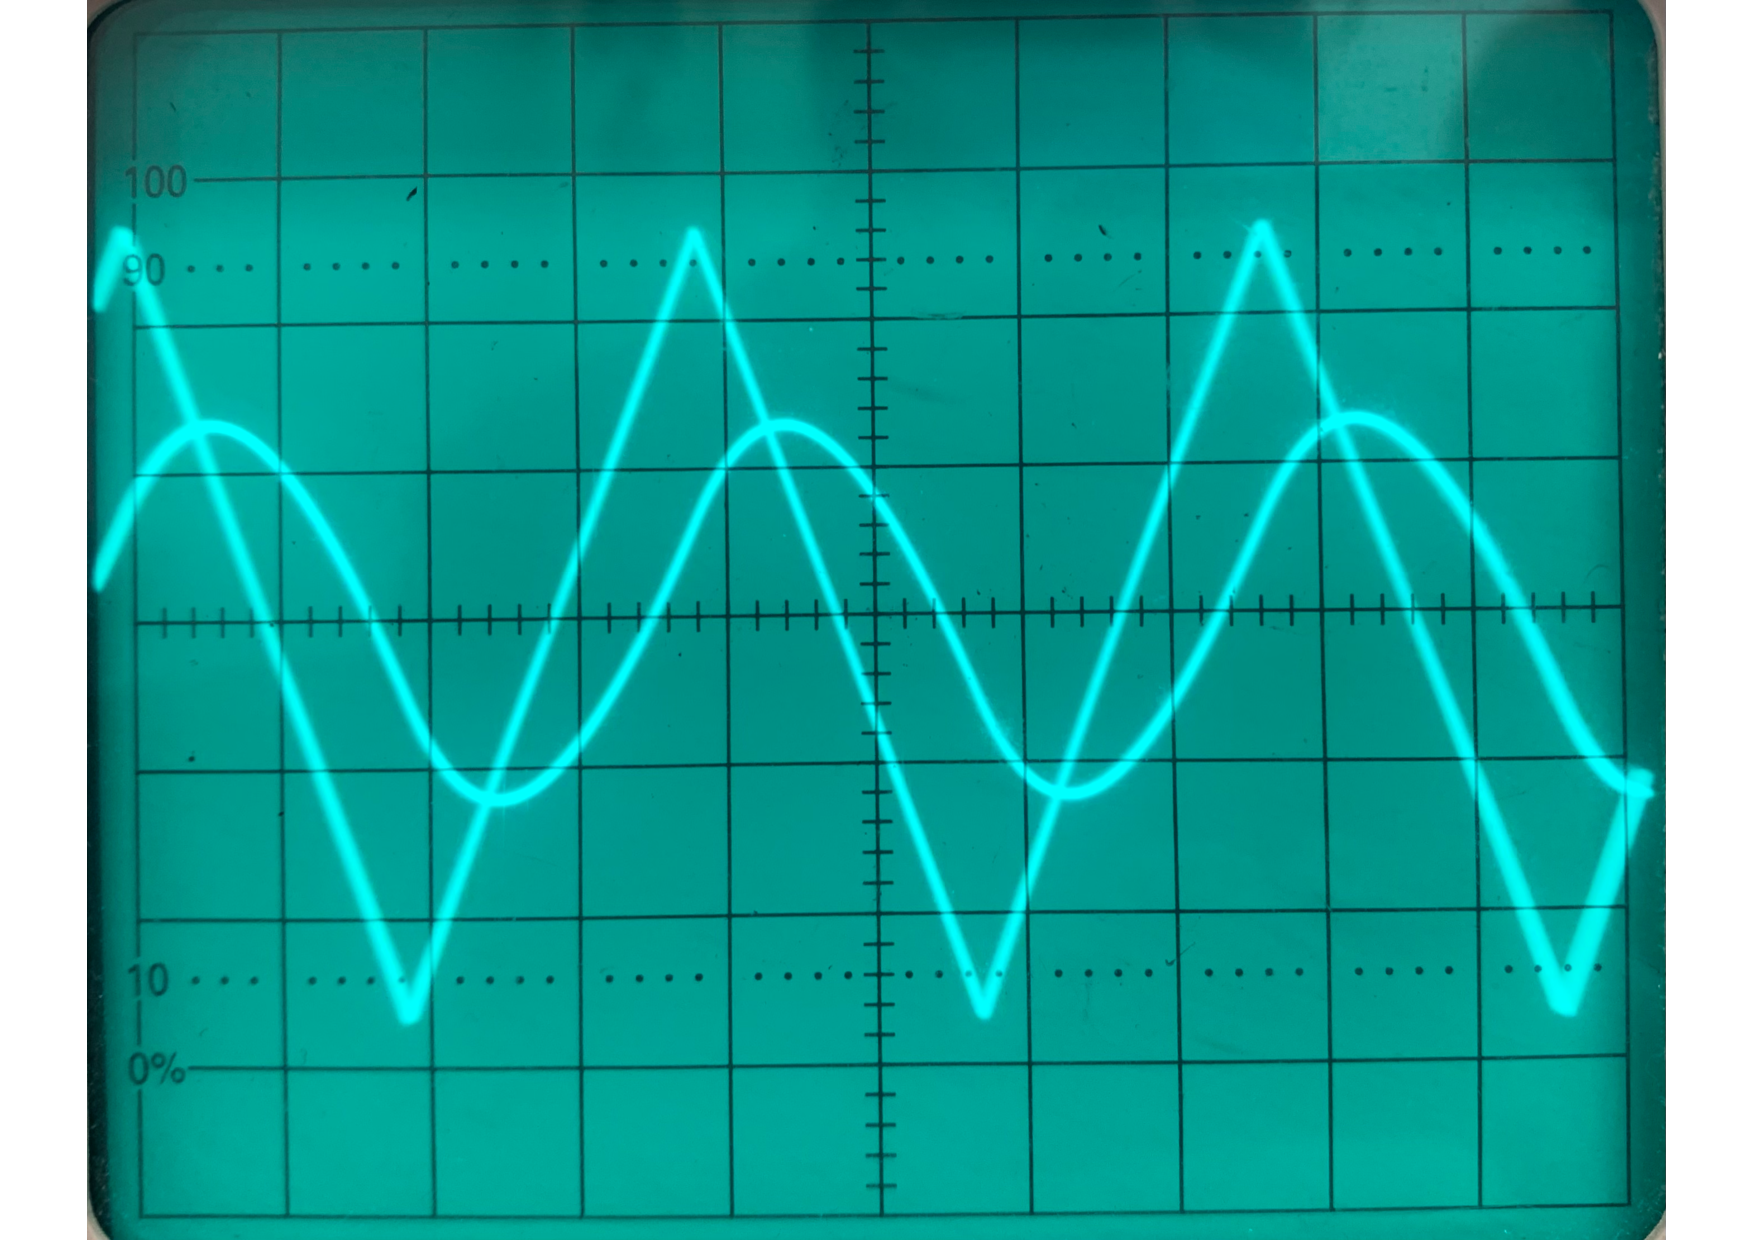
\includegraphics[height=8cm]{content/Aufgabe d - Dreieckspannung.pdf}
  \caption{Dreieckspannung $U_{0}$ und Kondensatorspannung mit $f=5$kHz.}
  \label{fig:aufgabe d - dreieckspannung}
\end{figure}

\begin{figure}
  \centering
  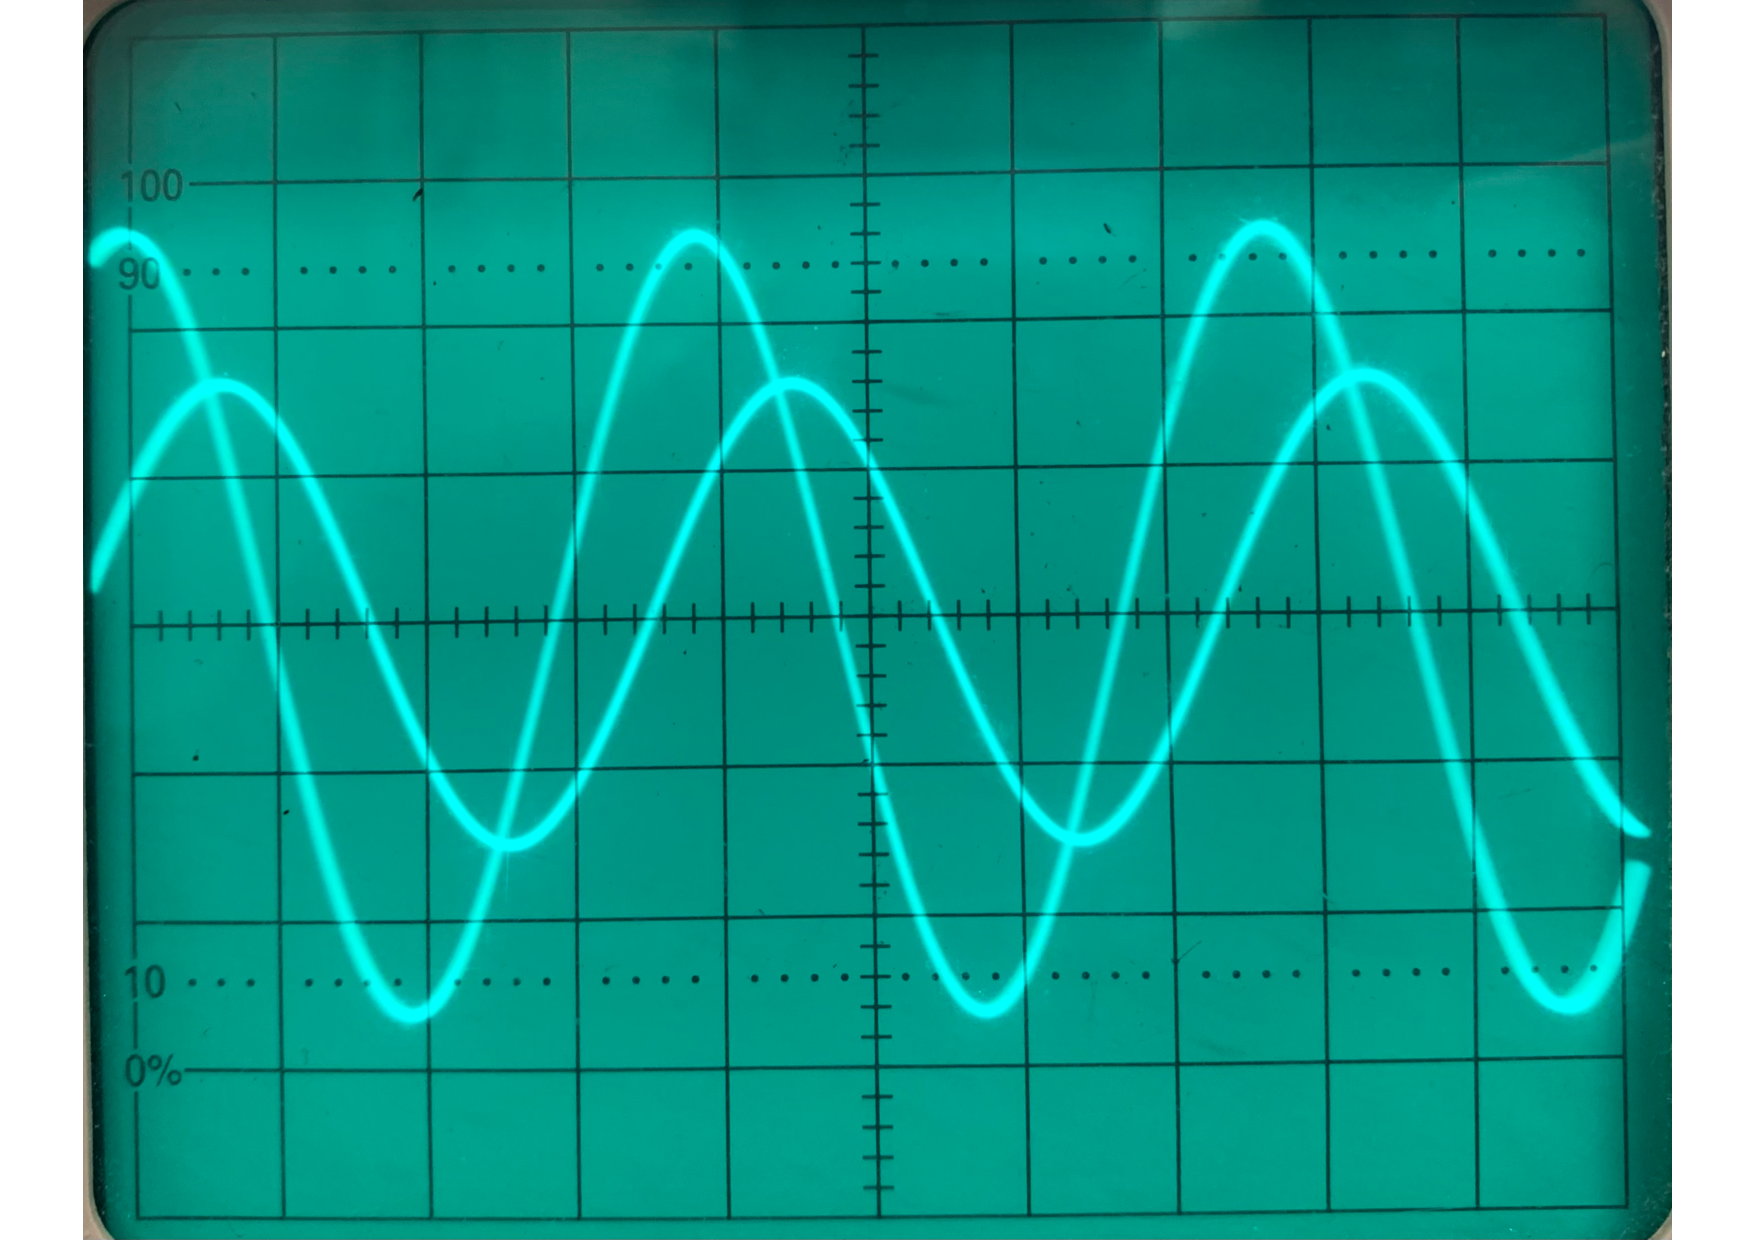
\includegraphics[height=8cm]{content/Aufgabe d - Sinusspannung.pdf}
  \caption{Sinusspannung $U_{0}$ und Kondensatorspannung mit $f=5$kHz.}
  \label{fig:aufgabe d - sinusspannung}
\end{figure}
